% Chapter 4

\chapter{Architecture}

\label{ch:architecture}

%----------------------------------------------------------------------------------------

\section{Overview}\label{sec:overview}

Tangible is implemented as a single Python package, without any external
dependencies.

The architecture of Tangible can be categorized into four different parts: The
abstract syntax tree (AST), code generation backends, shapes and utils.

\begin{figure}[h]
	\centering
	\definecolor{BackendsColor}{RGB}{116,143,204}
\definecolor{AstColor}{RGB}{199,108,107}
\definecolor{ShapesColor}{RGB}{227,225,107}
\definecolor{UtilsColor}{RGB}{118,219,125}

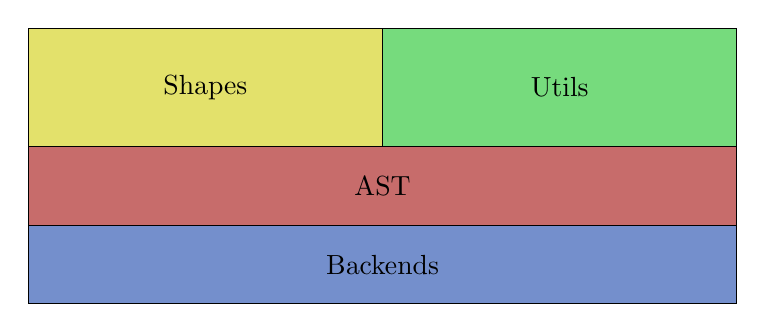
\begin{tikzpicture}
	\filldraw [fill=BackendsColor] (0,0) rectangle node [align=center] {Backends} (9,1) ;
	\filldraw [fill=AstColor] (0,1) rectangle node [align=center] {AST} (9,2);
	\filldraw [fill=ShapesColor] (0,2) rectangle node [align=center] {Shapes} (4.5,3.5);
	\filldraw [fill=UtilsColor] (4.5,2) rectangle node [align=center] {Utils} (9,3.5);
\end{tikzpicture}

	\caption{Architecture Diagram}
	\label{img:architecture}
\end{figure}

%----------------------------------------------------------------------------------------

\section{AST}\label{sec:ast}

The \texttt{ast.py} module provides the objects for the abstract syntax tree
(AST) for Tangible. It contains the following classes:

\subsection{Base class}

\begin{itemize}
	\item \texttt{AST}: The base shape for all AST elements.
\end{itemize}

\subsection{2D shapes}

\begin{itemize}
	\item \texttt{Circle}: A circle shape with a specified radius.
	\item \texttt{CircleSector}: A circle sector shape (pizza slice) with a
		specified radius and angle.
	\item \texttt{Rectangle}: A rectangular shape with a specified width and
		height.
	\item \texttt{Polygon}: A polygon shape made from a list of 2D coordinates.
\end{itemize}

\subsection{3D shapes}

\begin{itemize}
	\item \texttt{Cube}: A cube with a specified width, height and depth.
	\item \texttt{Sphere}: A sphere with a specified radius.
	\item \texttt{Cylinder}: A cylinder with a height and top/bottom radii.
	\item \texttt{Polyhedron}: An arbitrary 3D shape made from connected triangles
		or quads.
\end{itemize}

\subsection{Transformations}

\begin{itemize}
	\item \texttt{Translate}: Used to translate an object.
	\item \texttt{Rotate}: Used to rotate an object.
	\item \texttt{Scale}: Used to scale an object.
	\item \texttt{Mirror}: Used to mirror an object.
\end{itemize}

\subsection{Boolean Operations}

\begin{itemize}
	\item \texttt{Union}: Combine multiple shapes into a single shape.
	\item \texttt{Difference}: A boolean difference of two or more shapes.
	\item \texttt{Intersection}: A boolean intersection of two or more shapes.
\end{itemize}

\subsection{Extrusions}

\begin{itemize}
	\item \texttt{LinearExtrusion}: Extrude a 2D object linearly along the z axis.
	\item \texttt{RotateExtrusion}: Extrude a 2D object around the z axis. 
\end{itemize}

%----------------------------------------------------------------------------------------

\section{Backends}\label{sec:backends}

%----------------------------------------------------------------------------------------

\section{Shapes}\label{sec:shapes}

%----------------------------------------------------------------------------------------

\section{Utils}\label{sec:utils}
